% !TEX encoding = UTF-8
% Supplemental Material for DKAP Paper — PeerJ Computer Science
% Section cross-references renumbered to match paper/PeerJ_CS/main.tex (2026-07-14)
\documentclass[10pt,a4paper]{article}
\usepackage[utf8]{inputenc}
\usepackage{cite}
\usepackage{amsmath,amssymb}
\usepackage{bm}
\usepackage{graphicx}
\usepackage{float}
\usepackage{booktabs}
\usepackage{multirow}
\usepackage{array}
\usepackage{url}
\usepackage[hidelinks]{hyperref}
\usepackage{enumitem}
\usepackage[margin=2.5cm]{geometry}
\usepackage{longtable}

\newcolumntype{L}[1]{>{\raggedright\arraybackslash}p{#1}}
\newcolumntype{C}[1]{>{\centering\arraybackslash}p{#1}}
\newcolumntype{R}[1]{>{\raggedleft\arraybackslash}p{#1}}

\title{Supplementary Material:\\Completeness over Structuring: A Controlled Text-to-SQL Ablation and Source-Code Analysis of Twenty-Nine AI Systems}
\author{Dooil Kwak}
\date{}

\begin{document}
\emergencystretch=3em
\maketitle

\tableofcontents
\newpage

%% ============================================================
%%  S1: MULTI-AGENT INTER-RATER RELIABILITY
%% ============================================================
\section{Inter-Rater Reliability Assessment}
\label{sec:interrater}

We validate the DKS/RSS rubric at two complementary levels: a \emph{cross-family} study across seven independent model lineages (primary evidence; Section~\ref{sec:crossfamily}), and a \emph{within-family} study with five personas of a single base model (secondary, an upper bound on reproducibility; Section~\ref{sec:withinfamily}). The two estimate different quantities---cross-lineage generalizability versus within-lineage reproducibility---and should not be read as one number ``dropping'' to another.

\subsection{Cross-Family Generalizability Study}
\label{sec:crossfamily}

Seven LLM judges drawn from independent model families and lineages---OpenAI GPT-5.4, Anthropic Claude Sonnet~4.6, Google Gemini~3.1~Pro, Mistral Medium~3.5, DeepSeek~V3.2, Alibaba Qwen3.6-27B, and Zhipu GLM-5.2---independently scored thirteen of the sixteen external systems on the refined DKS/RSS rubric (temperature~$=0$; one neutral expert persona per model; consensus aggregation). These are exactly the external systems in the final analysis for which structured source-code evidence was available; the remaining three (AutoGPT, Haystack, Rasa) were author-scored only and are excluded here. Genuine lineage diversity is what turns agreement into evidence of rubric clarity rather than shared-model bias; for this reason Moonshot Kimi was excluded (its K2 architecture reuses the DeepSeek-V3 design), as was Meta Llama (no post-2025 release on the serving platform). Component scores were clamped to the rubric range $[0,\text{max}]$ (2 of $7\,\text{judges}\times13\,\text{systems}\times13\,\text{rubric components}=1{,}183$ adjusted; 0 parse failures). All thirteen systems are open-source, so the study is fully reproducible via \texttt{experiments/openrouter\_crossfamily\_ira.py}; internal industrial systems are excluded because confidential code cannot be sent to external judge APIs.

\begin{table}[h]
\centering
\caption{Cross-family agreement (seven lineages, thirteen external systems).}
\begin{tabular}{@{}lll@{}}
\toprule
Metric & Value & Interpretation \\
\midrule
Krippendorff's $\alpha$ (interval) & 0.718 & Acceptable (tentative; $\alpha\geq0.667$) \\
Mean pairwise Spearman $\rho$ & 0.782 & Strong rank agreement \\
Mean pairwise Cohen's $\kappa$ & 0.656 & Substantial \\
Fleiss' $\kappa$ (4-bin) & 0.367 & Moderate (coarse binning) \\
Author--ensemble Spearman $\rho$ & 0.786 ($p=0.002$) & Substantial \\
Author--ensemble Pearson $r$ & 0.851 ($p<0.001$) & Strong \\
\bottomrule
\end{tabular}
\end{table}

\begin{table}[h]
\centering
\caption{Per-system ensemble DKS+RSS totals across the seven families.}
\begin{tabular}{@{}lrrrr@{}}
\toprule
System & Mean & Min & Max & SD \\
\midrule
MedRAG & 8.0 & 8 & 8 & 0.0 \\
CrewAI & 17.1 & 2 & 31 & 8.3 \\
LlamaIndex & 25.6 & 17 & 36 & 5.6 \\
BIRD-SQL & 17.9 & 13 & 22 & 3.5 \\
Wheatley & 29.4 & 19 & 37 & 6.2 \\
FinSQL & 39.4 & 32 & 65 & 10.6 \\
SpeechBrain & 39.4 & 10 & 53 & 13.7 \\
AudioCraft & 20.4 & 10 & 32 & 8.7 \\
EmotiVoice & 45.0 & 36 & 56 & 6.5 \\
GraphRAG & 54.3 & 43 & 60 & 5.3 \\
MetaGPT & 33.4 & 28 & 39 & 4.3 \\
DeepTutor & 31.7 & 26 & 40 & 5.0 \\
PulseAI & 21.1 & 18 & 23 & 1.7 \\
\bottomrule
\end{tabular}
\end{table}

The families differ in absolute generosity (per-family mean totals: OpenAI 36.1, Google 33.5, Anthropic 29.5, GLM 28.9, Mistral 28.3, DeepSeek 27.6, Qwen 22.2) yet rank systems consistently (pairwise Spearman 0.58--0.91). This absolute/rank dissociation is exactly what is expected of a \emph{relative complexity descriptor}: judges disagree on how strict to be but agree on which systems encode more structured domain knowledge. Divergence is largest for boundary systems (e.g., SpeechBrain, range 10--53; FinSQL, range 32--65), consistent with the residual-divergence note in the main text.

\subsection{Within-Family Reproducibility (Single Base Model --- Upper Bound)}
\label{sec:withinfamily}

As a secondary check on internal reproducibility, we employed an LLM-as-Judge protocol with five persona-differentiated raters instantiated from a single base model (Qwen3-32B-AWQ, served via vLLM). Because all five raters share one lineage, the resulting agreement is an \emph{upper bound} on reproducibility, not a measure of evaluator independence. Each agent was assigned a distinct professional background designed to elicit diverse rubric interpretations:

\begin{enumerate}
\item \textbf{Software Architect} (12+ years system design): Strict on D4 (Schema) and RSS; distinguishes retrieval from model inference.
\item \textbf{ML Researcher} (NeurIPS/ACL reviewer): More generous on D2 (Ontology) for graph-based systems; careful about D1 glossary requirements.
\item \textbf{Data Engineer} (10 years ETL/DW): Practical on D1 and D4; strict on D8 (Regulatory) and R3 (Permissions).
\item \textbf{Cross-Domain Specialist} (healthcare/fintech): Strict on D3 (cross-ontology); generous on D8 when domain constraints are encoded as operational rules.
\item \textbf{Junior Developer} (3 years): Literal rubric interpretation; conservative baseline scorer.
\end{enumerate}

Each agent independently scored ten external systems using the refined DKS/RSS rubric (Section~\ref{sec:rubric_refinements}). Temperature was set to 0.0 for deterministic output. Agents received identical system evidence summaries extracted from source code analysis but no access to the author's scores. Two systems from the original twelve-system cohort (LLaVA, Logic-LLM) were subsequently removed from the final 13-pair configuration; three systems added later (MetaGPT, Pulse AI, DeepTutor) were scored by the author alone. All kappa statistics below are computed on the ten systems present in both the agent cohort and the final analysis.

\subsection{Rubric Refinements}

\label{sec:rubric_refinements}

Based on disagreement analysis from a preliminary single-rater assessment ($\kappa = 0.52$), the following clarifications were added to the rubric before multi-agent scoring:

\begin{itemize}
\item \textbf{D1 (Lexicon)}: ``Count only \textit{explicitly declared} domain terms in dedicated glossary files, configuration constants, enum values, or docstring dictionaries. Variable names in code do NOT count unless part of a curated list. Typed field constants in data model classes (e.g., Pydantic/dataclass fields) count if they define domain entity attributes.''
\item \textbf{D2 (Ontology/KG)}: ``Only \textit{semantic} graphs where nodes represent domain concepts and edges represent domain relationships (is-a, part-of, causes). Computational graphs (GNN edges, attention layers) do NOT count unless they encode domain-semantic relationships.''
\item \textbf{D4 (Schema/DDL)}: ``Includes SQL DDL, JSON Schema, YAML configs with typed fields, Protocol Buffers, or Python dataclasses/Pydantic models that define domain entities with typed attributes. Pure Python classes with only methods (no typed fields) do NOT count.''
\item \textbf{D6 (Rules)}: ``Includes LLM-orchestrated procedural rules (e.g., iterative extraction loops, budget-based truncation, graph pruning). Programming language patterns count only if they encode domain-specific semantics.''
\item \textbf{R2 (Vector Search)}: ``Neural feature extraction for model inference (e.g., CLIP encoding for VLM, mel-spectrogram for TTS) does NOT count as vector search.''
\end{itemize}

Three worked examples were included in the rubric prompt: MedRAG (D1=0, no glossary file), FinSQL (D1=10, 1,170 financial column names), and GraphRAG (D4=10, 7 data model classes with typed fields).

For framework systems (LlamaIndex), the evidence summary included the directive: ``Score as a TYPICAL PRODUCTION DEPLOYMENT, not the framework ceiling.''

\subsection{Summary Statistics}

\begin{table}[H]
\centering
\caption{Multi-Agent Inter-Rater Reliability Summary}
\label{tab:irr_summary}
\begin{tabular}{@{}lll@{}}
\toprule
\textbf{Metric} & \textbf{Value} & \textbf{Interpretation} \\
\midrule
Fleiss' $\kappa$ (4-bin) & 0.933 & Almost perfect \\
Mean pairwise Cohen's $\kappa$ & 0.989 & Almost perfect \\
Mean Spearman $\rho$ & 0.934 & Almost perfect \\
ICC(2,k) Total & 0.972 & Excellent \\
ICC(2,k) DKS & 0.975 & Excellent \\
ICC(2,k) RSS & 0.965 & Excellent \\
\midrule
R1 vs Agent Mean $\rho$ & 0.704 ($p=0.023$) & Moderate--substantial \\
R1 vs Agent Mean $\kappa$ & 0.819 & Almost perfect \\
R1 vs Agent Mean $|\Delta|$ & 7.8 & -- \\
\bottomrule
\end{tabular}
\end{table}

\subsection{Per-System Scores}

\begin{table}[H]
\centering
\caption{Per-System DKS+RSS Scores: Author (R1) vs.\ Five Agent Raters}
\label{tab:irr_persystem}
\footnotesize
\setlength{\tabcolsep}{3pt}
\begin{tabular}{@{}lrrrrrrrr@{}}
\toprule
\textbf{System} & \textbf{R1} & \textbf{SWA} & \textbf{MLR} & \textbf{DE} & \textbf{DS} & \textbf{JD} & \textbf{Mean} & \textbf{$\sigma$} \\
\midrule
\multicolumn{9}{@{}l}{\scriptsize\textit{Original inter-rater cohort (10 systems currently in analysis):}} \\
MedRAG      & 10 &  8 &  8 &  8 &  8 &  8 &  8.0 & 0.0 \\
CrewAI      & 24 & 13 & 14 & 16 & 14 & 14 & 14.2 & 1.0 \\
LlamaIndex  & 27 & 47 & 41 & 39 & 33 & 33 & 38.6 & 5.3 \\
BIRD-SQL    & 29 & 21 & 19 & 21 & 20 & 18 & 19.8 & 1.2 \\
Wheatley    & 35 & 47 & 47 & 47 & 47 & 47 & 47.0 & 0.0 \\
FinSQL      & 41 & 36 & 36 & 36 & 38 & 38 & 36.8 & 1.0 \\
SpeechBrain & 41 & 46 & 46 & 46 & 51 & 46 & 47.0 & 2.0 \\
AudioCraft  & 46 & 34 & 34 & 34 & 34 & 34 & 34.0 & 0.0 \\
EmotiVoice  & 50 & 36 & 46 & 41 & 46 & 46 & 43.0 & 4.0 \\
GraphRAG    & 65 & 64 & 59 & 64 & 57 & 58 & 60.4 & 3.0 \\
\midrule
\multicolumn{9}{@{}l}{\scriptsize\textit{New systems (author-scored, post-study; agent scores not available):}} \\
MetaGPT     & 41 & --- & --- & --- & --- & --- & --- & --- \\
Pulse AI    & 15 & --- & --- & --- & --- & --- & --- & --- \\
DeepTutor   & 48 & --- & --- & --- & --- & --- & --- & --- \\
\bottomrule
\multicolumn{9}{@{}l}{\scriptsize SWA=SW Architect, MLR=ML Researcher, DE=Data Engineer,} \\
\multicolumn{9}{@{}l}{\scriptsize DS=Domain Specialist, JD=Junior Developer. R1=Author score.} \\
\end{tabular}
\end{table}

\subsection{Pairwise Agreement Matrix}

\begin{table}[H]
\centering
\caption{Pairwise Cohen's $\kappa$ (Quadratic-Weighted, 4-bin)}
\label{tab:pairwise_kappa}
\footnotesize
\begin{tabular}{@{}lccccc@{}}
\toprule
 & \textbf{SWA} & \textbf{MLR} & \textbf{DE} & \textbf{DS} & \textbf{JD} \\
\midrule
SWA & --- & 1.000 & 1.000 & 0.946 & 1.000 \\
MLR &     & ---   & 1.000 & 1.000 & 1.000 \\
DE  &     &       & ---   & 0.946 & 1.000 \\
DS  &     &       &       & ---   & 1.000 \\
JD  &     &       &       &       & --- \\
\bottomrule
\multicolumn{6}{@{}l}{\scriptsize Mean pairwise $\kappa = 0.989$.} \\
\end{tabular}
\end{table}

\subsection{Divergence Analysis: R1 vs.\ Agent Scores}

Three systems account for the majority of the R1--Agent divergence (ranked by $|\Delta|$):

\textbf{Wheatley (R1=35, Agent Mean=47.0, $|\Delta|=12.0$).} Agents interpreted RL signal pre-processing (job feature extraction, graph construction) as domain knowledge structuring (L2), yielding higher D2/D4 scores. The author scored these as computational graph operations rather than semantic domain artifacts. This reflects the ambiguity of distinguishing domain-semantic graphs from computational-graph structures in RL systems.

\textbf{AudioCraft (R1=46, Agent Mean=34.0, $|\Delta|=12.0$).} The author scored richer genre/audio processing profiles (D5: 10/10 for 100+ audio profiles) than agents, who applied a narrower literal interpretation of ``domain profiles'' and scored D5 lower. This reflects the rubric's tension between audio engineering configurations and semantic domain profiles.

\textbf{LlamaIndex (R1=27, Agent Mean=38.6, $|\Delta|=11.6$).} The author scored using a ``typical deployment'' methodology (DKS$=$20), discounting framework capabilities not typically activated in production (e.g., PropertyGraphIndex, EntityExtractor). Despite the ``score as typical deployment'' instruction, agents still scored some framework capabilities as present. The remaining gap (27 vs.\ 38.6) reflects the inherent ambiguity of scoring framework systems.

\textbf{GraphRAG (R1=65, Agent Mean=60.4, $|\Delta|=4.6$, rank 8/10).} After rubric refinement, this gap narrowed substantially from the preliminary assessment ($\Delta=29 \to \Delta=4.6$). The remaining difference is in D6 (R1=7 for LLM-orchestrated procedural rules; Agent Mean$\approx$3--5) and D7 (R1=3 for configurable language parameter; agents=0, requiring explicit multilingual dictionaries).

\subsection{Limitations of LLM-as-Judge}

The within-family raters all share one base model (Qwen3-32B-AWQ), so their near-perfect agreement may partly reflect shared model biases rather than genuine rubric clarity. Specifically: (1) the model may systematically under- or over-score certain component types (e.g., all agents gave AudioCraft RSS=0, unanimously interpreting neural conditioning as non-retrieval); (2) persona differentiation, while producing measurable scoring variation (the Junior Developer persona tends to score at or near the lowest, $\bar{x}=34.2$ vs.\ overall $\bar{x}=34.9$ across the ten analysis systems), may not fully replicate the interpretive diversity of human experts. This is precisely why the cross-family study (Section~\ref{sec:crossfamily}) is the primary evidence: drawing judges from seven independent lineages substantially removes the shared-model confound, and the agreement that survives ($\alpha=0.718$, $\rho=0.782$) is therefore attributable to rubric clarity rather than a common prior. A human inter-rater study with independent domain experts would still strengthen validation and remains future work.

\subsection{Layer-Assignment Agreement (L1--L5)}
\label{sec:layer_agreement}

The five-layer decomposition was validated separately from DKS scoring (this is the ``full breakdown'' referenced in the main paper's construct-validity discussion). Five independent personas (single base model) assigned each of the $N=92$ pipeline stages---decomposed from the thirteen paradigm-matched external systems---to one of the five layers, reaching Fleiss' $\kappa = 0.937$ (91.3\% full consensus). Because a five-class agreement statistic could in principle be high while the single load-bearing boundary (L2$\to$L3) is contested, we isolate that boundary: of the 92 stages, 42 carry an L2 or L3 consensus (22 L2, 20 L3), and on this subset the five raters still reach Fleiss' $\kappa = 0.819$ (83.3\% full consensus), with only five L2$\leftrightarrow$L3 cross-assignments among the 210 labels. As expected, the producer--consumer boundary is the \textit{harder} split---its agreement is lower than the global $0.937$, and four of the eight stages with any disagreement involve an L2-vs-L3 call---yet agreement remains substantial, indicating that the boundary the framework rests on is itself reliably identifiable, not merely the easy L1/L4/L5 distinctions. The complete per-system stage-to-layer mapping is provided in the public data release (Data Availability).


%% ============================================================
%%  S2: B2' INFORMATION CONTROL EXPERIMENT
%% ============================================================
\section{\texorpdfstring{B2$'$}{B2'} Information Control Experiment}
\label{sec:b2prime_detail}

\subsection{Prompt Design}

The B2$'$ prompt provides identical domain knowledge to DKAP but in unstructured narrative prose. Token counts were matched within 2\%:

\begin{itemize}
\item \textbf{DKAP}: ${\sim}$1,960 tokens --- structured markdown tables with column-level type/domain annotations, explicit join rules, semantic glossary with coded values, column transform rules.
\item \textbf{B2$'$}: ${\sim}$1,920 tokens --- continuous narrative describing the same tables, columns, types, relationships, and domain semantics without tables, headers, or structured formatting.
\end{itemize}

Both prompts contain: (1) all five table definitions with column names, types, and constraints; (2) all foreign key relationships and join conditions; (3) the semantic glossary (VIP codes, credit ratings, payment status codes); (4) value-domain rules (KRW amounts, YYYYMMDD dates, ratio ranges). The B2$'$ prompt additionally includes elaborative reasoning hints (e.g., ``When performing joins across tables, always include both the member ID and reference month in the JOIN condition'') that arise naturally from narrative exposition but are absent from DKAP's tabular format.

\subsection{Error Analysis: Hard Question Divergence}

Of 18 Hard questions, B2$'$ and DKAP agree on 16 (10 both correct, 6 both wrong). Two questions diverge:

\textbf{Q21} (3-table JOIN + HAVING, ``total spending per member with VIP grade and credit rating, filtered by 1M KRW threshold''):
\begin{itemize}
\item \textbf{DKAP error}: Omitted \texttt{m.customer\_name} from SELECT and GROUP BY. The gold SQL includes it. DKAP's structured schema marks this column as ``Domain: PII,'' which may have suppressed the LLM's inclination to include it in output.
\item \textbf{B2$'$ correct}: Included \texttt{m.customer\_name} as expected.
\end{itemize}

\textbf{Q29} (Window function + cumulative sum, ``rank members by spending with cumulative total''):
\begin{itemize}
\item \textbf{DKAP error}: Converted window function to GROUP BY aggregation (\texttt{GROUP BY usage\_rank}), losing per-member granularity.
\item \textbf{B2$'$ correct}: Used \texttt{RANK() OVER} plus \texttt{SUM() OVER} with frame \texttt{ROWS BETWEEN UNBOUNDED} \texttt{PRECEDING AND CURRENT ROW}.
\end{itemize}

\textbf{Interpretation.} Neither error reflects a systematic failure of structured prompting. Q21's column omission (possibly influenced by PII annotation) and Q29's aggregation-type confusion are isolated cases. The 2/18 divergence is small relative to the sample size and does not suggest a systematic pattern.

\subsection{Stochastic Robustness: Full Results}

\begin{table}[H]
\centering
\caption{Stochastic Results by Difficulty (temp=0.3, 5 runs, Finance 50Q)}
\label{tab:stochastic_full}
\footnotesize
\begin{tabular}{@{}llrrrrr@{}}
\toprule
\textbf{Cond.} & \textbf{Diff.} & \textbf{R1} & \textbf{R2} & \textbf{R3} & \textbf{R4} & \textbf{R5} \\
\midrule
B2       & Easy   & 90.0 & 90.0 & 100.0 & 90.0 & 90.0 \\
B2       & Medium & 60.0 & 60.0 & 70.0 & 60.0 & 70.0 \\
B2       & Hard   & 16.7 & 22.2 & 16.7 & 22.2 & 22.2 \\
\midrule
B2$'$    & Easy   & 90.0 & 90.0 & 90.0 & 90.0 & 100.0 \\
B2$'$    & Medium & 90.0 & 90.0 & 90.0 & 80.0 & 80.0 \\
B2$'$    & Hard   & 55.6 & 55.6 & 66.7 & 55.6 & 55.6 \\
\midrule
DKAP     & Easy   & 100.0 & 100.0 & 100.0 & 100.0 & 100.0 \\
DKAP     & Medium & 90.0 & 90.0 & 90.0 & 90.0 & 80.0 \\
DKAP     & Hard   & 55.6 & 50.0 & 50.0 & 50.0 & 50.0 \\
\bottomrule
\end{tabular}
\end{table}

Key observations: (1) DKAP achieves 100\% on Easy across all 5 runs (zero variance); (2) B2's Hard performance is the most volatile (range: 16.7--22.2\%); (3) DKAP's overall $\sigma = 0.9$ is the lowest across conditions, directionally consistent with a stabilization effect though not statistically distinguishable at $n=5$ (cf.\ the main-text caveat).


%% ============================================================
%%  CROSS-MODEL ABLATION DETAIL
%% ============================================================
\section{Cross-Model Ablation: Per-Difficulty and Per-Seed Detail}
\label{sec:crossmodel_detail}

This section provides the breakdown behind the cross-model generalization result (the Cross-Model Generalization subsection of the main paper): six independent model families $\times$ three conditions $\times$ ten seeds $\times$ 50 finance queries $=9{,}000$ runs at temperature~$0.3$, scored by execution accuracy (EX). The ablation uses six model families; the cross-family reliability study (Section~\ref{sec:interrater}) uses seven judge lineages (adding GLM-5.2) for evaluator diversity, a distinct role that need not share the same model set. The structuring null reported here is therefore finance-specific---the only domain with a B2$'$ control. The evaluation script and the derived per-run statistics are in the data release (\texttt{experiments/openrouter\_ablation.py}); the raw 14\,MB generations log (\texttt{generations.jsonl}) is regenerable by re-running that script and is available on request.

\begin{table}[h]
\centering
\caption{Cross-model per-difficulty execution accuracy (\%) by condition (mean over ten seeds; E/M/H $=$ Easy/Medium/Hard).}
\label{tab:crossmodel_diff}
\footnotesize
\begin{tabular}{@{}llrrr@{}}
\toprule
Model & Cond & E & M & H \\
\midrule
OpenAI GPT-5.4 & B2 & 100.0 & 73.7 & 31.7 \\
 & B2$'$ & 100.0 & 94.2 & 60.0 \\
 & DKAP & 100.0 & 92.6 & 55.0 \\
\midrule
Anthropic Claude Sonnet 4.6 & B2 & 100.0 & 72.1 & 31.1 \\
 & B2$'$ & 100.0 & 90.0 & 64.4 \\
 & DKAP & 100.0 & 92.1 & 65.6 \\
\midrule
Google Gemini 3.1 Pro & B2 & 98.5 & 68.9 & 23.9 \\
 & B2$'$ & 100.0 & 81.6 & 36.7 \\
 & DKAP & 99.2 & 89.5 & 37.2 \\
\midrule
DeepSeek V3.2 & B2 & 87.7 & 55.8 & 27.2 \\
 & B2$'$ & 100.0 & 87.9 & 45.0 \\
 & DKAP & 100.0 & 88.4 & 49.4 \\
\midrule
Qwen3.6-27B & B2 & 96.9 & 68.4 & 24.4 \\
 & B2$'$ & 97.7 & 82.1 & 50.0 \\
 & DKAP & 100.0 & 83.7 & 53.3 \\
\midrule
Mistral Medium 3.5 & B2 & 99.2 & 58.9 & 25.0 \\
 & B2$'$ & 100.0 & 94.7 & 48.3 \\
 & DKAP & 100.0 & 90.5 & 49.4 \\
\bottomrule
\end{tabular}
\end{table}

Across all six families the structure is the same: the large gain is B2$\to$B2$'$ (completeness), concentrated on Medium and Hard queries, while DKAP$-$B2$'$ (structuring, information held fixed) is small and inconsistent in sign. Per-difficulty structuring gains are near zero on Easy (all conditions saturate) and show no consistent direction on Medium/Hard---e.g., Google $+7.9$pp on Medium versus OpenAI $-1.6$ and Mistral $-4.2$; OpenAI $-5.0$pp on Hard versus DeepSeek $+4.4$. No difficulty band yields a systematic structuring advantage across models, consistent with the near-zero aggregate ($+0.7$pp, 95\% CI $[-1.0,+3.0]$) reported in the main paper. These per-cell deltas are descriptive only---uncorrected for the eighteen family$\times$difficulty comparisons---and no individual cell is read as an inference; the sole inferential statement is the aggregate CI.

\begin{table}[h]
\centering
\caption{Cross-model output stability: standard deviation of execution accuracy (\%) across the ten seeds, by condition. DKAP's seed-to-seed variance is at or below B2's for five of six families (the exception is OpenAI, $2.4$ vs.\ $2.2$); it is the lowest of the three conditions for three families (Google, Qwen, Mistral) and tied-lowest for a fourth (Anthropic).}
\label{tab:crossmodel_var}
\footnotesize
\begin{tabular}{@{}lrrr@{}}
\toprule
Model & B2 $\sigma$ & B2$'$ $\sigma$ & DKAP $\sigma$ \\
\midrule
OpenAI GPT-5.4 & 2.2 & 2.0 & 2.4 \\
Anthropic Claude Sonnet 4.6 & 2.0 & 1.3 & 1.3 \\
Google Gemini 3.1 Pro & 3.1 & 1.9 & 1.8 \\
DeepSeek V3.2 & 2.9 & 1.7 & 1.8 \\
Qwen3.6-27B & 3.3 & 3.8 & 1.8 \\
Mistral Medium 3.5 & 2.9 & 1.8 & 1.7 \\
\bottomrule
\end{tabular}
\end{table}

This cross-model output-variance pattern (DKAP at or below B2 for five of six families; lowest of the three conditions for three) echoes the directional variance reduction observed on the primary model (the B2$'$ stochastic-robustness analysis above). As in the main text, we report it as a directional stabilization signal rather than a confirmed guarantee, since the per-family differences are small relative to the ten-seed sampling error.


%% ============================================================
%%  S3: DKS/RSS SCORING SHEET
%% ============================================================
\section{DKS and RSS Rubric Definitions}
\label{sec:supp_rubric}
The full component-level thresholds for the Domain Knowledge Score (DKS) and Retrieval Sophistication Score (RSS) rubrics---summarized in the main paper (Section~3.4)---are given below.

\begin{table}[t]
\centering
\caption{Domain Knowledge Score (DKS) Rubric. All thresholds are grounded in countable code artifacts (file entry counts, node/edge counts, table/FK counts, regex pattern counts). See the main paper, Section~3.4, for concrete scoring examples.}
\label{tab:dks_rubric}
\small
\begin{tabular}{@{}llp{4.2cm}@{}}
\toprule
\textbf{Component} & \textbf{Max} & \textbf{Criteria (quantitative anchors)} \\
\midrule
D1: Domain lexicon & 15 & 0: none $|$ 5: 1--50 terms $|$ 10: 51--200 ($\log_2$ scale) $|$ 15: $>$200 \\
D2: Ontology/KG & 15 & 0: none $|$ 5: flat ($<$50 nodes) $|$ 10: hierarchical ($<$200) $|$ 15: graph ($\geq$200, edges$\geq$0.5$\times$nodes) \\
D3: Cross-ontology & 10 & 0: none $|$ 5: single standard $|$ 10: multi-standard (e.g., ICD+SNOMED) \\
D4: Schema/DDL & 15 & 0: none $|$ 5: 1--5 tables $|$ 10: 6--15 tables+FK $|$ 15: $>$15 tables+constraints \\
D5: Domain profiles & 10 & 0: none $|$ 3: $<$10 configs $|$ 6: 10--50 $|$ 10: $>$50 profiles \\
D6: Rule patterns & 10 & 0: none $|$ 3: $<$10 regex/rules $|$ 6: 10--30 $|$ 10: $>$30 patterns \\
D7: Multi-language & 10 & 0: single lang $|$ 5: bilingual $|$ 10: trilingual+ \\
D8: Regulatory & 15 & 0: none $|$ 5: basic PII $|$ 10: sector reg $|$ 15: multi-regulation \\
\bottomrule
\end{tabular}
\end{table}

\begin{table}[t]
\centering
\caption{Retrieval Sophistication Score (RSS) Rubric}
\label{tab:rss_rubric}
\small
\begin{tabular}{@{}llp{4.0cm}@{}}
\toprule
\textbf{Component} & \textbf{Max} & \textbf{Criteria} \\
\midrule
R1: Intent classification & 3 & 0: none $|$ 1: keyword $|$ 2: ML $|$ 3: multi-stage \\
R2: Vector search & 3 & 0: none $|$ 1: flat $|$ 2: filtered $|$ 3: search+reranking \\
R3: Permission filtering & 2 & 0: none $|$ 1: role-based $|$ 2: document+role \\
R4: Multi-index fusion & 2 & 0: single $|$ 1: dual $|$ 2: triple+ \\
R5: Adaptive routing & 2 & 0: fixed $|$ 1: rule-based $|$ 2: ML/LLM-based \\
\bottomrule
\end{tabular}
\end{table}

\section{Supporting Figures: DKS--Complexity Correlation and Cross-Validation}

This section provides two figures supporting analyses reported in the main paper: the DKS+RSS--complexity correlation (Fig.~\ref{fig:scatter}) and the paired internal--external cross-validation (Fig.~\ref{fig:crossval}).

\begin{figure}[!t]
\centering
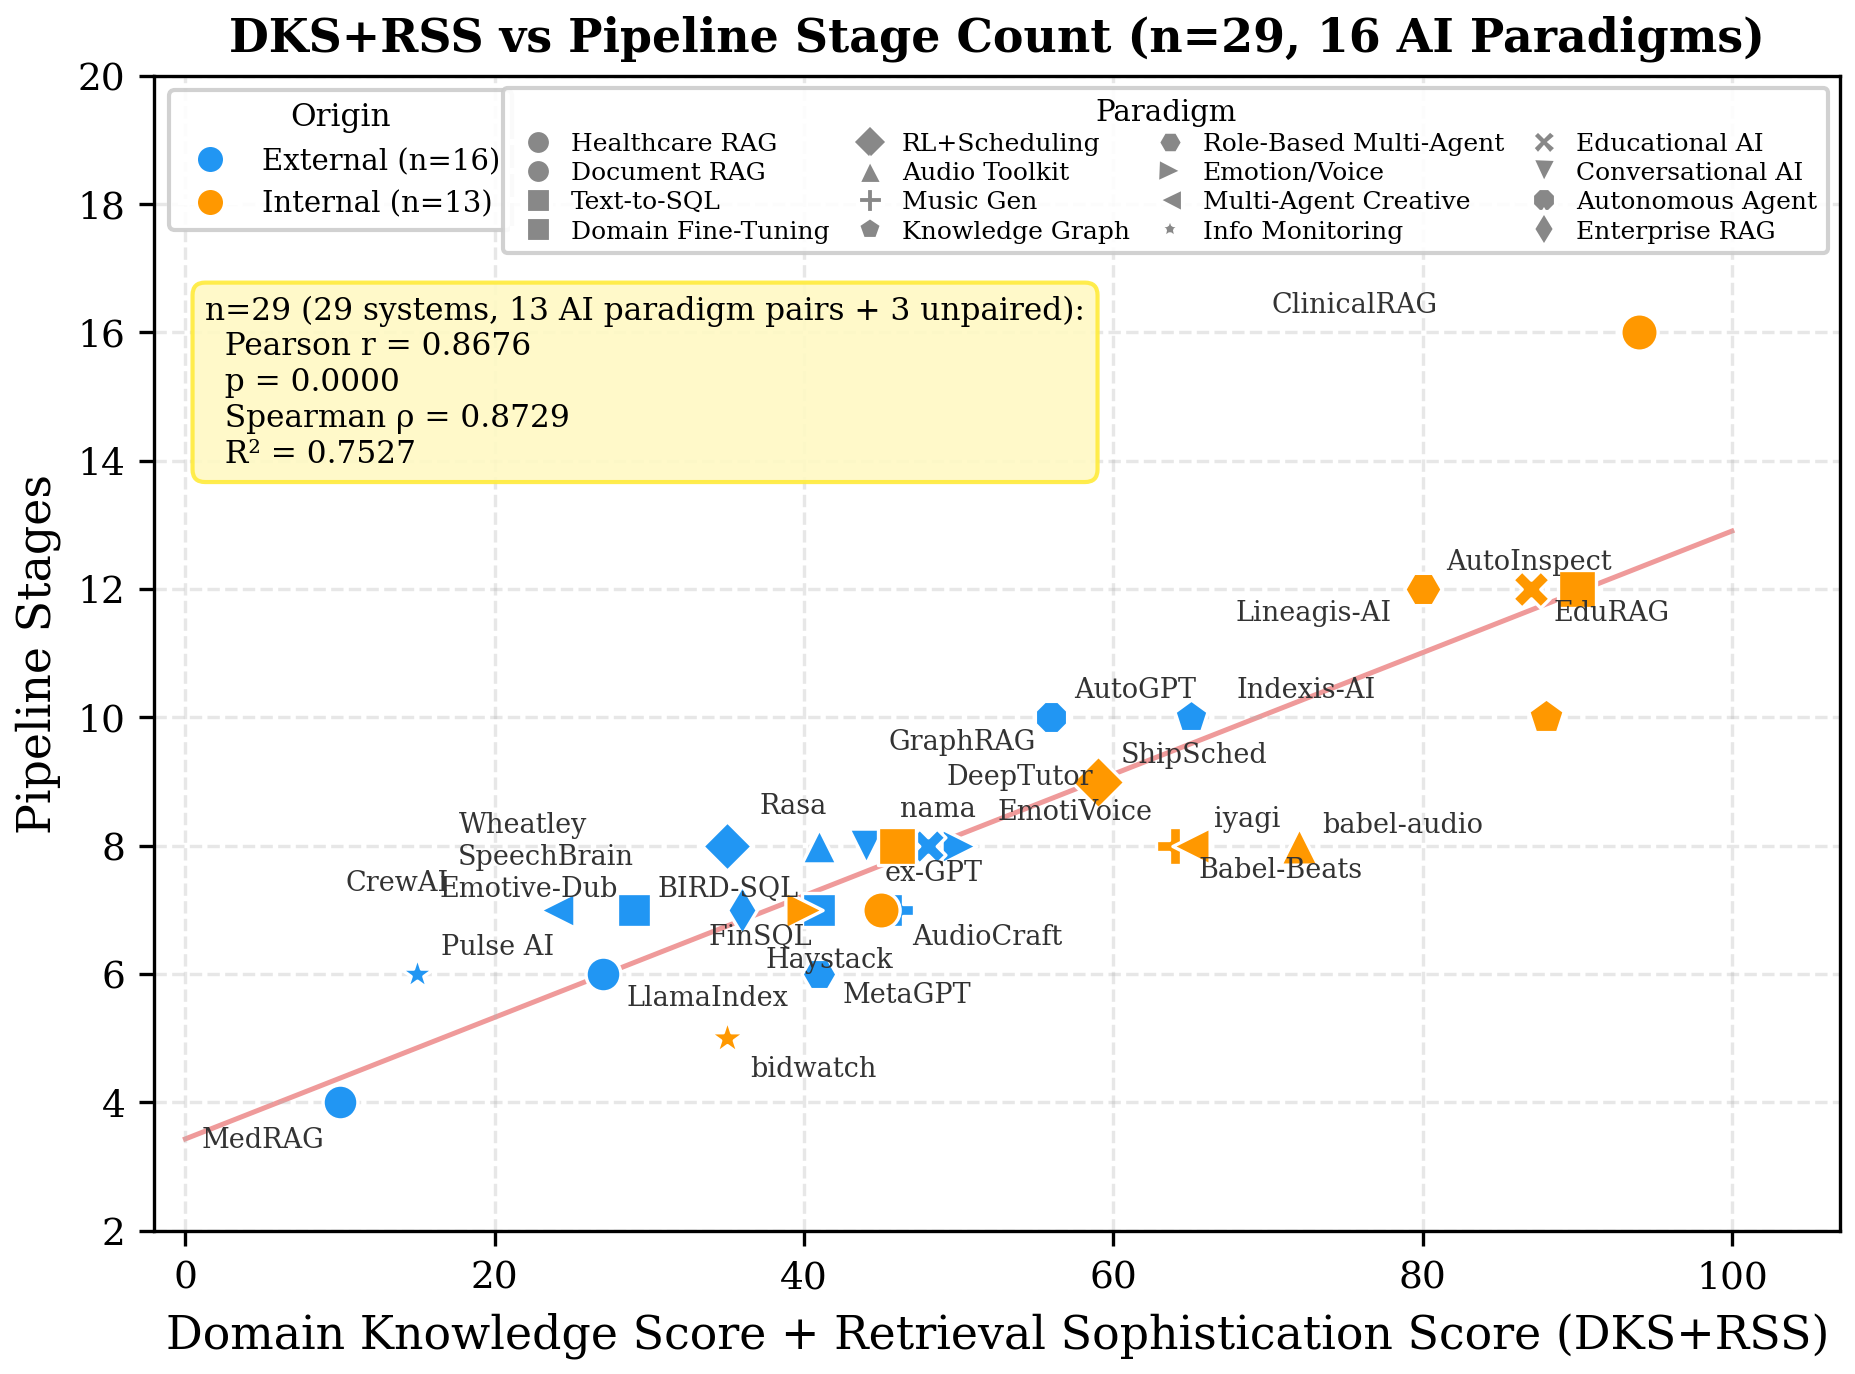
\includegraphics[width=\textwidth]{fig3_24systems_scatter.png}
\caption{DKS+RSS versus pipeline stage count for twenty-nine AI systems. A significant positive association is observed: Pearson $r = 0.868$ ($p < 0.001$, $R^2 = 0.753$); Spearman $\rho = 0.873$ ($p < 0.001$). External-only ($n=16$): $r = 0.857$ (95\% CI [0.63, 0.95], $p < 0.001$, $R^2 = 0.734$). DKS+RSS is a researcher-defined score; across seven independent LLM judge lineages ($n=13$ external systems) it shows Krippendorff's $\alpha = 0.718$ (mean pairwise $\rho = 0.782$) and author--ensemble rank correlation $\rho = 0.786$ ($p = 0.002$); see the main paper, Section~5.7.4.}
\label{fig:scatter}
\end{figure}

\begin{figure}[!t]
\centering
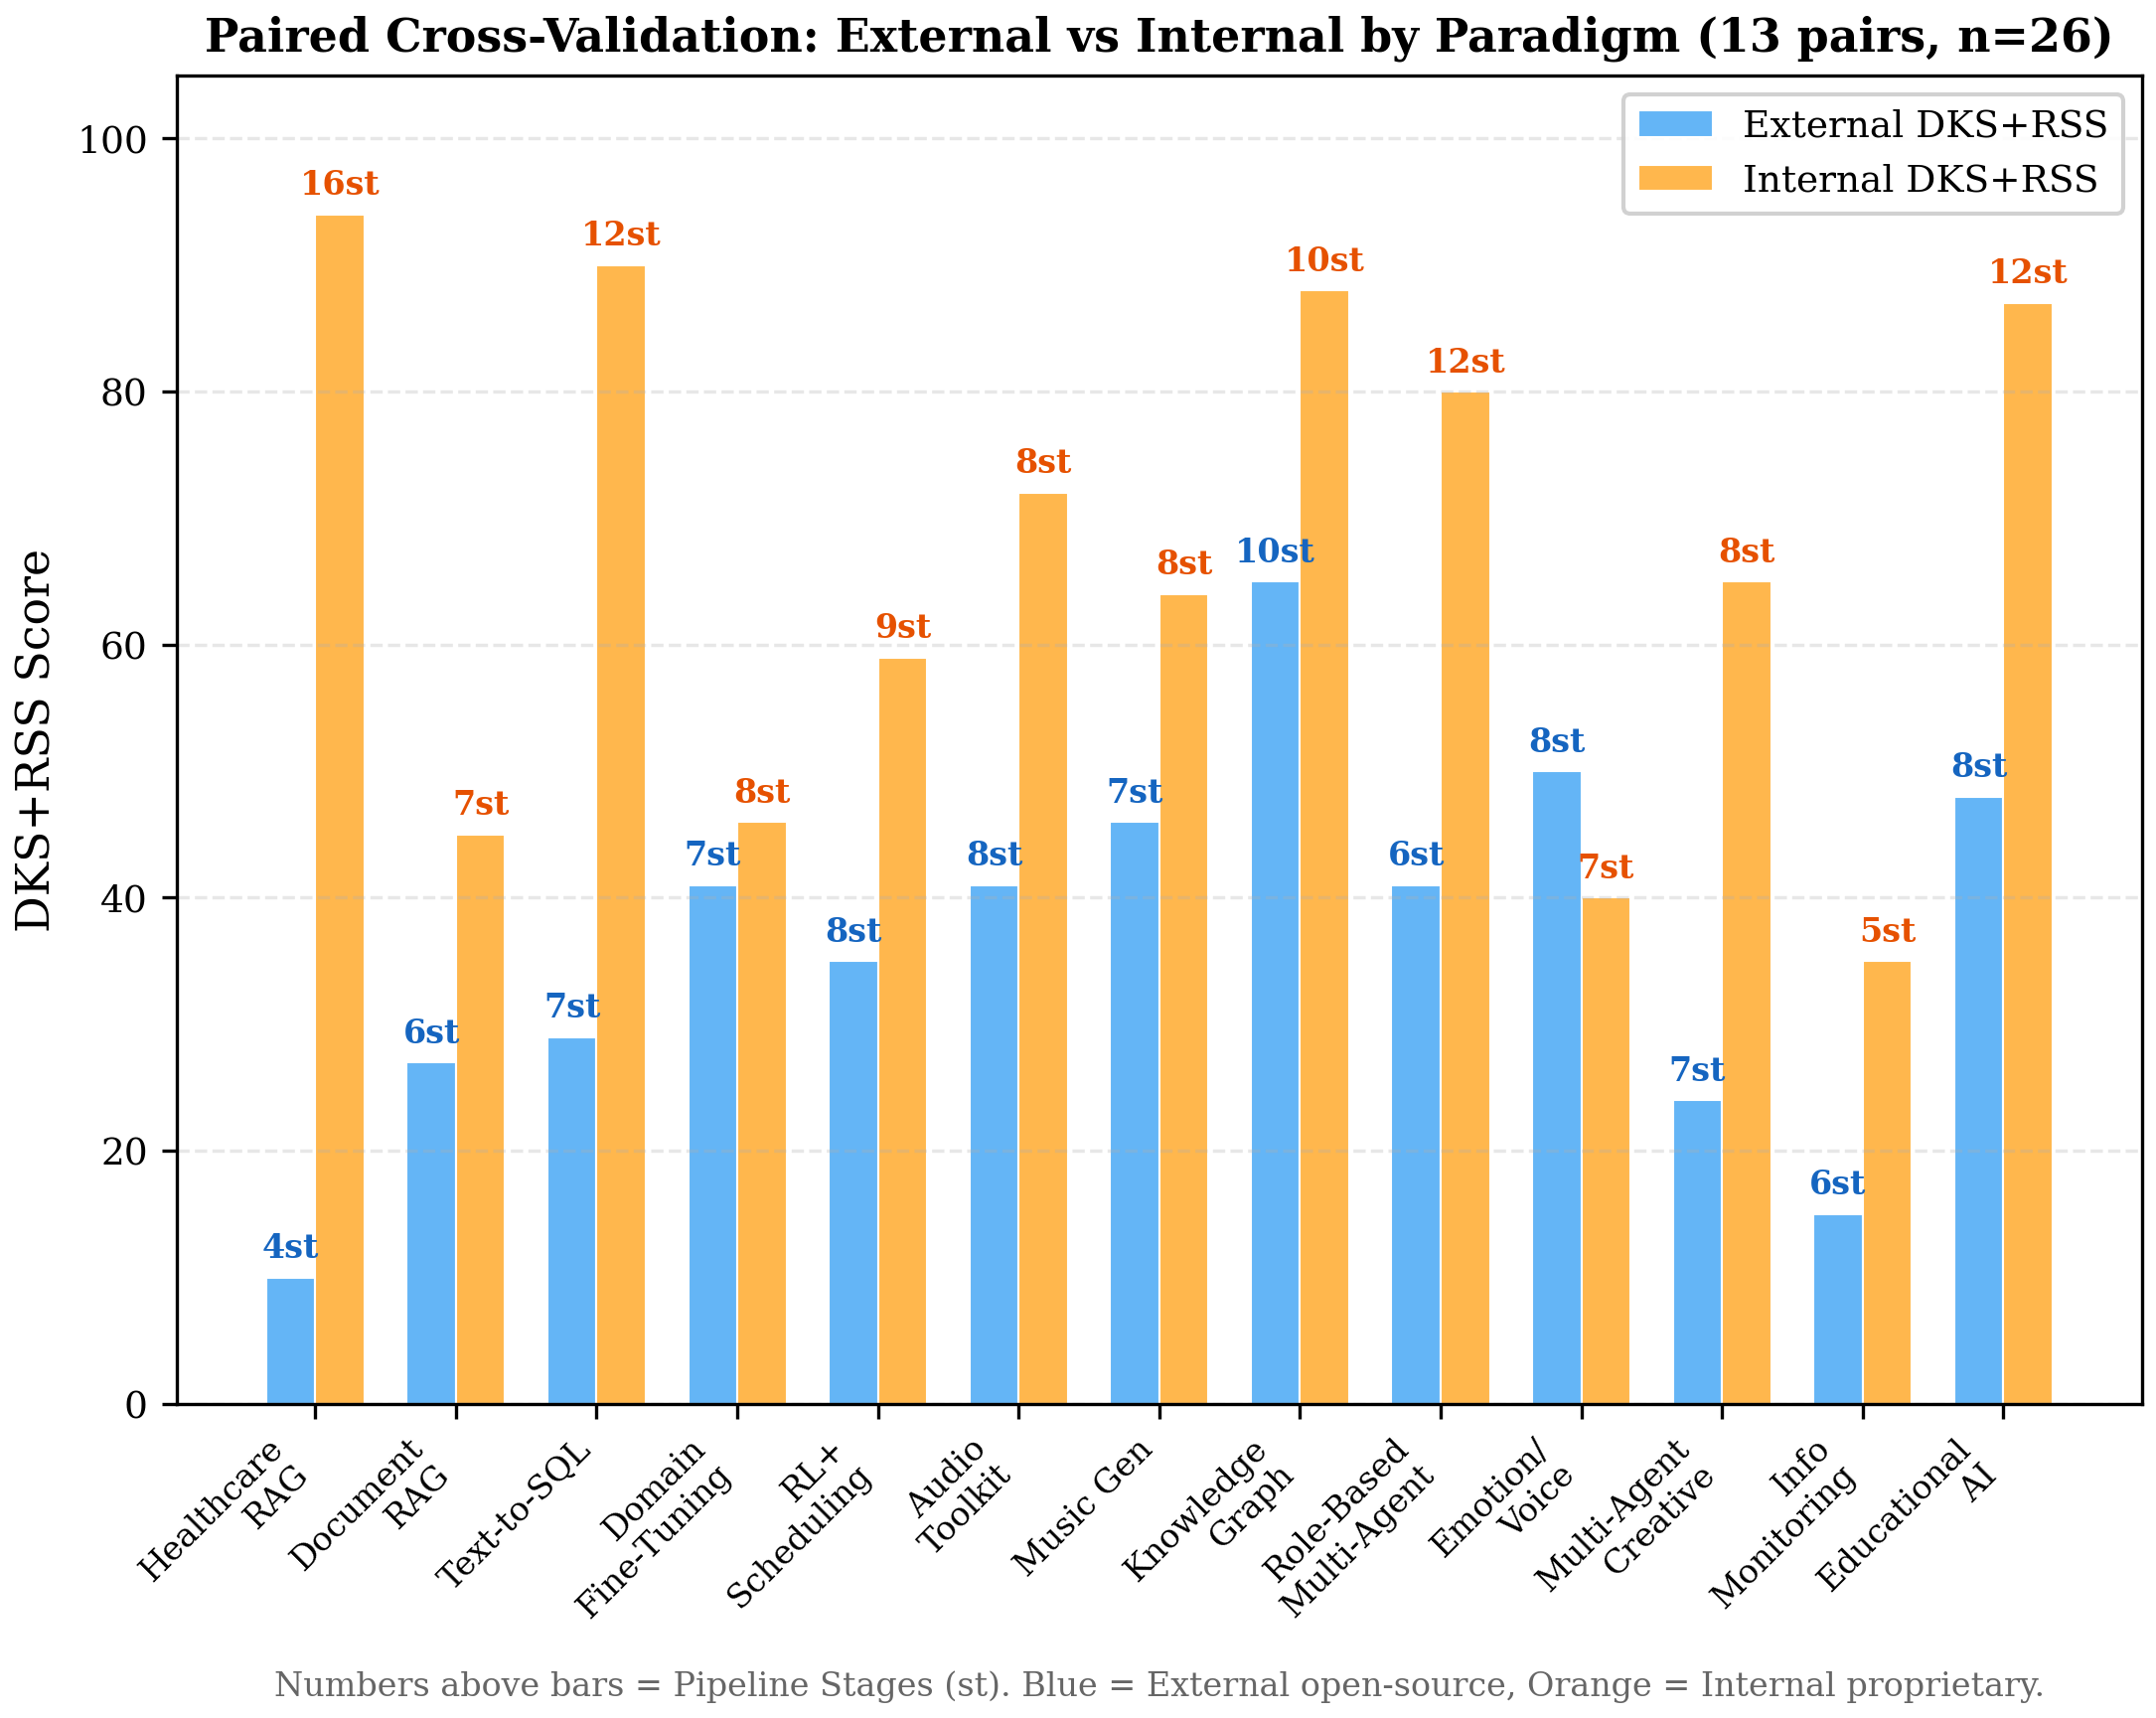
\includegraphics[width=0.94\textwidth]{fig4_paired_crossvalidation.png}
\caption{Paired cross-validation between thirteen external and thirteen internal systems matched by AI paradigm. Internal systems score higher in 12/13 pairs (mean difference $+30.2$), reflecting production deployment requirements (security, audit, multi-language, regulatory compliance) that systematically amplify L2 complexity. One reversal: Emotion/Voice (EmotiVoice 50 $>$ Emotive-Dub 40). Wilcoxon $W = 2.0$, $p < 0.001$ (two-sided), indicating a statistically significant difference.}
\label{fig:crossval}
\end{figure}

\section{Per-Domain and Stochastic Result Tables}

Detailed per-condition results for the healthcare and public-procurement domains, and the per-seed stochastic-robustness table, are provided below; the finance results and the cross-domain summary appear in the main paper.

\begin{table*}[!t]
\centering
\caption{Healthcare Clinical QA Results (Qwen3-32B-AWQ, N=40$\times$3). EX/EM by difficulty: E=Easy (n=12), M=Medium (n=14), H=Hard (n=14).}
\label{tab:healthcare_results}
\footnotesize
\begin{tabular}{@{}lrrrrrrr@{}}
\toprule
\textbf{Cond.} & \textbf{EX\%} & \textbf{EM\%} & \textbf{EXEC\%} & \textbf{Lat.} & \textbf{EX-E} & \textbf{EX-M} & \textbf{EX-H} \\
\midrule
B1  & 2.5  & 2.5  & 2.5   & 415\,ms  & 8.3  & 0.0  & 0.0  \\
B2  & 57.5 & 12.5 & 87.5  & 1151\,ms & 75.0 & 64.3 & 35.7 \\
DKAP& 70.0 & 7.5$^\dagger$  & 100.0 & 739\,ms  & \textbf{100.0} & \textbf{78.6} & \textbf{35.7} \\
\bottomrule
\multicolumn{8}{@{}l}{\scriptsize $^\dagger$EM reversal vs.\ B2 on Easy queries; see text.} \\
\end{tabular}
\end{table*}

\begin{table}[t]
\centering
\caption{Public Procurement Results (Qwen3-32B-AWQ, N=25$\times$3)}
\label{tab:public_results}
\footnotesize
\begin{tabular}{@{}lrrrr@{}}
\toprule
\textbf{Condition} & \textbf{EX\%} & \textbf{EM\%} & \textbf{EXEC\%} & \textbf{Lat.(ms)} \\
\midrule
B1: Vanilla LLM  & 0.0  & 0.0 & 0.0  & 368 \\
B2: Flat-chunk RAG & 64.0 & 8.0 & 84.0 & 604 \\
DKAP (Proposed)  & 64.0 & 8.0 & 96.0 & 697 \\
\bottomrule
\end{tabular}
\end{table}

\begin{table}[t]
\centering
\caption{Stochastic Robustness (Finance, 50Q, temp$=$0.3, 5 runs). 95\% bootstrap CI for $\sigma$ computed from $n=5$ runs (50{,}000 resamples); wide CIs reflect small $n$.}
\label{tab:stochastic}
\small
\begin{tabular}{@{}lrrl@{}}
\toprule
\textbf{Condition} & \textbf{Mean EX\%} & $\bm{\sigma}$ & \textbf{95\% CI$_\sigma$} \\
\midrule
B2            & 55.6 & 2.2 & [0.0, 3.0] \\
B2$'$         & 78.0 & 1.4 & [0.0, 2.0] \\
DKAP          & 78.4 & \textbf{0.9} & [0.0, 1.1] \\
\bottomrule
\end{tabular}
\end{table}

\section{Full Per-System DKS/RSS and Stage Counts (Twenty-Nine Systems)}

The complete per-system scores for all twenty-nine analyzed systems, sorted by DKS+RSS, are listed below (system citations appear in the main paper).

\begin{table}[t]
\centering
\caption{Overview of Twenty-Nine Analyzed Systems (13 Internal + 16 External$^\dagger$), sorted by DKS+RSS. System names in the table are space-abbreviated forms of the full names used in the text (e.g., EmotiVce $=$ EmotiVoice, SpchBrain $=$ SpeechBrain, LlamaIdx $=$ LlamaIndex, Emot-Dub $=$ Emotive-Dub, babel-aud $=$ babel-audio).}
\label{tab:all_systems}
\small
\setlength{\tabcolsep}{4pt}
\begin{tabular*}{\textwidth}{@{\extracolsep{\fill}}rllrrrrlr@{}}
\toprule
\textbf{\#} & \textbf{System} & \textbf{Orig} & \textbf{DKS} & \textbf{RSS} & \textbf{Tot} & \textbf{St} & \textbf{Engine} & \textbf{Paradigm} \\
\midrule
1  & MedRAG$^\dagger$     & Ext & 5  & 5  & 10 &  4 & LLM+RAG   & Hlth RAG  \\
2  & Pulse AI$^\dagger$  & Ext & 14 & 1  & 15 &  6 & LLM       & InfoMon   \\
3  & CrewAI$^\dagger$    & Ext & 15 & 9  & 24 &  7 & LLM Agt   & Multi-Agt \\
4  & LlamaIdx$^\dagger$ & Ext & 20 & 7  & 27 &  6 & LLM RAG   & Doc RAG   \\
5  & BIRD-SQL$^\dagger$  & Ext & 26 & 3  & 29 &  7 & LLM+T5    & Txt2SQL   \\
6  & bidwatch            & Int & -- & -- & 35 &  5 & LLM       & InfoMon   \\
7  & Wheatley$^\dagger$ & Ext & 33 & 2  & 35 &  8 & RL+GNN    & RL+Sched  \\
8  & Haystack$^\dagger$ & Ext & 26 & 10 & 36 &  7 & LLM RAG   & EntRAG    \\
9  & Emot-Dub            & Int & -- & -- & 40 &  7 & LLM       & Emo/V     \\
10 & FinSQL$^\dagger$    & Ext & 35 & 6  & 41 &  7 & LLM+LoRA  & DomFT     \\
11 & MetaGPT$^\dagger$   & Ext & 37 & 4  & 41 &  6 & LLM Agt   & RoleMAgt  \\
12 & SpchBrain$^\dagger$ & Ext & 37 & 4  & 41 &  8 & ASR/TTS   & Speech    \\
13 & Rasa$^\dagger$         & Ext & 39 & 5  & 44 &  8 & BERT+ML   & ConvAI    \\
14 & ex-GPT              & Int & -- & -- & 45 &  7 & LLM       & Doc RAG   \\
15 & AudioCrft$^\dagger$ & Ext & 42 & 4  & 46 &  7 & Trans.LM  & MusGen    \\
16 & nama                & Int & -- & -- & 46 &  8 & LLM       & DomFT     \\
17 & DeepTutor$^\dagger$ & Ext & 42 & 6  & 48 &  8 & LLM+RAG   & Edu AI    \\
18 & EmotiVce$^\dagger$ & Ext & 47 & 3  & 50 &  8 & BERT+TTS  & Emo/V     \\
19 & AutoGPT$^\dagger$   & Ext & 51 & 5  & 56 & 10 & LLM Agt   & AutAgent  \\
20 & ShipSched           & Int & -- & -- & 59 &  9 & RL+LLM    & RL+Sched  \\
21 & Babel-Bts           & Int & -- & -- & 64 &  8 & LLM       & MusGen    \\
22 & GraphRAG$^\dagger$ & Ext & 57 & 8  & 65 & 10 & LLM+KG    & KG/Graph  \\
23 & iyagi               & Int & -- & -- & 65 &  8 & LLM Agt   & Multi-Agt \\
24 & babel-aud           & Int & -- & -- & 72 &  8 & ML        & Speech    \\
25 & AutoInspect         & Int & -- & -- & 80 & 12 & VLM       & RoleMAgt  \\
26 & EduRAG              & Int & -- & -- & 87 & 12 & LLM       & Edu AI    \\
27 & Indexis-AI          & Int & -- & -- & 88 & 10 & LLM+KG    & KG/Graph  \\
28 & Lineagis-AI         & Int & -- & -- & 90 & 12 & LLM       & Txt2SQL   \\
29 & ClinicalRAG         & Int & -- & -- & 94 & 16 & LLM+SQL   & Hlth RAG  \\
\bottomrule
\end{tabular*}
\par\smallskip
\parbox{\textwidth}{\footnotesize\raggedright
$^\dagger$Ext.\ open-source. 5 non-LLM: Wheatley, SpeechBrain, AudioCraft, EmotiVoice, Rasa. Tot=DKS+RSS, St=Stages.\\
--: proprietary system; per-component DKS/RSS breakdown not disclosed (client confidentiality). Tot source-mined, except three documentation-estimated systems (the main paper Section~5.7.4).}
\end{table}

\section{External-Systems Detail (LOC and Stage Counts)}

Table~\ref{tab:external_systems} reports the DKS+RSS scores, pipeline stages, Python LOC, and file counts for all sixteen external systems.

\begin{table}[!t]
\centering
\caption{DKS+RSS, Stages, and Python LOC for 16 External Systems}
\label{tab:external_systems}
\footnotesize
\setlength{\tabcolsep}{3pt}
\begin{tabular}{@{}rlrrrrll@{}}
\toprule
\# & \textbf{System} & \textbf{Tot} & \textbf{St} & \textbf{LOC} & \textbf{Fil} & \textbf{Paradigm} & \textbf{L?} \\
\midrule
1  & MedRAG      & 10 & 4  & 1.2K  & 8   & Hlth RAG  & Y \\
2  & Pulse AI    & 15 & 6  & 5.2K  & 26  & InfoMon   & Y \\
3  & CrewAI      & 24 & 7  & 213K  & 1K  & Multi-Agt & Y \\
4  & LlamaIdx    & 27 & 6  & 180K$^*$& 900$^*$& Doc RAG & Y \\
5  & BIRD-SQL    & 29 & 7  & 5.8K$^*$& 35$^*$& Txt2SQL & Y \\
6  & Wheatley    & 35 & 8  & 12K$^*$& 80$^*$& RL+Sched & N \\
7  & Haystack    & 36 & 7  & 62K   & 284 & EntRAG    & Y \\
8  & FinSQL      & 41 & 7  & 4.5K$^*$& 30$^*$& DomFT  & Y \\
9  & MetaGPT     & 41 & 6  & 89K   & 890 & RoleMAgt  & Y \\
10 & SpchBrain   & 41 & 8  & 95K$^*$& 450$^*$& Speech & N \\
11 & Rasa        & 44 &  8 & 60K   & 291 & ConvAI    & N \\
12 & AudioCrft   & 46 & 7  & 28K   & 175 & MusGen    & N \\
13 & DeepTutor   & 48 & 8  & 120K  & 582 & Edu AI    & Y \\
14 & EmotiVoice  & 50 & 8  & 15K$^*$& 90$^*$& Emo/V  & N \\
15 & AutoGPT     & 56 & 10 & 230K$^*$& 990$^*$& AutAgent & Y \\
16 & GraphRAG    & 65 & 10 & 50K   & 566 & KG/Graph  & Y \\
\bottomrule
\multicolumn{8}{@{}l}{\scriptsize Tot=DKS+RSS, St=Stages, Fil=Files, L?=LLM?} \\
\multicolumn{8}{@{}l}{\scriptsize $^*$Estimated from GitHub stats.} \\
\end{tabular}
\end{table}

\section{Cross-Paradigm RL Scheduling Illustration}
\label{sec:rl_note}

\textbf{Important methodological caveat.} The following RL comparison is \textit{not} an L2 ablation in the same sense as the LLM experiments above. It uses dispatching rule heuristics (B1: Random, B2: MWKR) as proxies for domain knowledge depth, and the full DKAP condition cannot be evaluated without dedicated RL re-training. We include this comparison as a qualitative illustration---not as cross-paradigm experimental evidence---and report it separately from the LLM ablation results.

Using the Wheatley RL-based Job Shop Scheduling (JSSP) system on three Taillard 15$\times$15 benchmark instances (ta01--ta03), we compare dispatching heuristics that differ in domain knowledge depth: B1 (Random: no domain features) versus B2 (MWKR: most-remaining-work heuristic, a single scheduling feature). The optimality gap reduces from 102.5\% (B1) to 30.9\% (B2), a $-$71.6pp improvement---the largest B1$\to$B2 step observed in this study. This directionally supports the hypothesis that even partial domain knowledge matters beyond LLM pipelines, but the dispatching-rule--to--L2 analogy is imperfect and this result should not be aggregated with the LLM ablation statistics.

\begin{table}[t]
\centering
\caption{LLM Ablation Summary (3 Domains). $\Delta$=DKAP$-$B2 except JSSP ($\Delta$=B1$-$B2 optimality gap reduction; qualitative illustration only, not L2 ablation).}
\label{tab:cross_paradigm}
\footnotesize
\begin{tabular}{@{}llrrrr@{}}
\toprule
\textbf{Domain} & \textbf{Eng.} & \textbf{B1} & \textbf{B2} & \textbf{DKAP} & $\Delta$ \\
\midrule
Finance    & LLM & 0.0 & 54.0 & 80.0 & $+$26.0 \\
Healthcare & LLM & 2.5 & 57.5 & 70.0 & $+$12.5 \\
Public     & LLM & 0.0 & 64.0 & 64.0 & $+$0.0 \\
\midrule
\multicolumn{6}{@{}l}{\scriptsize\textit{Qualitative note (not aggregated above):}} \\
JSSP$^\dagger$ & RL & 102.5\% & 30.9\% & --- & $-$71.6 \\
\bottomrule
\multicolumn{6}{@{}l}{\scriptsize All EX\% for LLM rows. $^\dagger$JSSP: optimality gap (\%), lower is better;} \\
\multicolumn{6}{@{}l}{\scriptsize $\Delta$=B1$-$B2; full DKAP requires RL re-training (future work).} \\
\end{tabular}
\end{table}

Across the three LLM domains, removing domain knowledge (B1) produces near-zero execution accuracy, and adding partial domain knowledge (B2) yields large improvements ($+$54.0pp to $+$64.0pp over B1). The full DKAP condition further improves over B2 in proportion to domain knowledge complexity (the main paper Section~4.4).

\textbf{Floor-effect caveat on B1.} B1$=$0.0\% in Finance and Public domains is a floor effect: the test queries require multi-table schema joins that zero-shot LLMs cannot resolve without any schema information, regardless of L2 design. B1 therefore provides only weak evidence for L2's architectural role; it establishes that domain knowledge is \textit{necessary}, not that structured organization is the specific mechanism. The architecturally informative comparison is DKAP vs.\ B2 ($+$26.0pp and $+$0.0pp), which controls for schema provision while varying only knowledge organization depth. The B1 baseline is reported for completeness and should not be interpreted as evidence that L2 absence alone causes performance collapse.



\section{DKS/RSS Scoring Sheet for Independent Raters}
\label{sec:scoring_sheet}

The following blank scoring template is provided for independent replication of the DKS/RSS assessment. Raters should clone each repository and examine source code directly, following the rubric criteria in Tables~\ref{tab:dks_rubric}--\ref{tab:rss_rubric} of this supplement (summarized in Section~3.4 of the main paper).

\subsection{Instructions}
\begin{enumerate}
\item Clone the repository and examine the source code.
\item Score each DKS component (D1--D8) independently using the rubric criteria.
\item Score each RSS component (R1--R5) independently.
\item Record a 1--2 sentence justification for each component score.
\item Do NOT reference any prior rater's scores.
\end{enumerate}

\subsection{Template}

For each system, complete the following:

\begin{center}
\footnotesize
\begin{tabular}{@{}lrl@{}}
\toprule
\textbf{Component} & \textbf{Score} & \textbf{Justification} \\
\midrule
D1: Domain lexicon (max 15) & \_\_\_ & \\
D2: Ontology/KG (max 15) & \_\_\_ & \\
D3: Cross-ontology (max 10) & \_\_\_ & \\
D4: Schema/DDL (max 15) & \_\_\_ & \\
D5: Domain profiles (max 10) & \_\_\_ & \\
D6: Rule patterns (max 10) & \_\_\_ & \\
D7: Multi-language (max 10) & \_\_\_ & \\
D8: Regulatory (max 15) & \_\_\_ & \\
\midrule
\textbf{DKS Total} & \_\_\_ / 100 & \\
\midrule
R1: Intent classification (max 3) & \_\_\_ & \\
R2: Vector search (max 3) & \_\_\_ & \\
R3: Permission filtering (max 2) & \_\_\_ & \\
R4: Multi-index fusion (max 2) & \_\_\_ & \\
R5: Adaptive routing (max 2) & \_\_\_ & \\
\midrule
\textbf{RSS Total} & \_\_\_ / 12 & \\
\midrule
\textbf{Pipeline Stage Count} & \_\_\_ & \\
\bottomrule
\end{tabular}
\end{center}

\subsection{Thirteen External Systems for Scoring}

\begin{enumerate}
\item \textbf{MedRAG}: \url{https://github.com/Teddy-XiongGZ/MedRAG} (ACL 2024 Findings)
\item \textbf{Pulse AI}: \url{https://github.com/tejiri-code/pulse-ai}
\item \textbf{CrewAI}: \url{https://github.com/crewAIInc/crewAI}
\item \textbf{LlamaIndex}: \url{https://github.com/run-llama/llama_index}
\item \textbf{BIRD-SQL}: \url{https://github.com/AlibabaResearch/DAMO-ConvAI} (bird/)
\item \textbf{Wheatley}: \url{https://github.com/jolibrain/wheatley} (CPAIOR 2024)
\item \textbf{FinSQL}: \url{https://github.com/bigbigwatermalon/FinSQL} (SIGMOD 2024)
\item \textbf{MetaGPT}: \url{https://github.com/FoundationAgents/MetaGPT} (ICLR 2024 Oral)
\item \textbf{SpeechBrain}: \url{https://github.com/speechbrain/speechbrain}
\item \textbf{AudioCraft}: \url{https://github.com/facebookresearch/audiocraft} (NeurIPS 2023)
\item \textbf{DeepTutor}: \url{https://github.com/HKUDS/DeepTutor}
\item \textbf{EmotiVoice}: \url{https://github.com/netease-youdao/EmotiVoice}
\item \textbf{GraphRAG}: \url{https://github.com/microsoft/graphrag}
\end{enumerate}

\noindent\textbf{Scoring notes for new systems:}
\begin{itemize}[nosep]
\item \textbf{MetaGPT} (DKS=37, RSS=4): D1=10 (role/SOP vocabulary), D2=5 (workflow graph), D3=0, D4=10 (schema for actions/messages), D5=6 (role profiles), D6=6 (constraint rules), D7=0, D8=0; R1=1, R2=2, R3=0, R4=0, R5=1.
\item \textbf{Pulse AI} (DKS=14, RSS=1): Minimal domain structuring; alert-monitoring pipeline with basic NLP. D1=5, D2=0, D3=0, D4=5, D5=4, D6=0, D7=0, D8=0; R1=1, R2=0, R3=0, R4=0, R5=0.
\item \textbf{DeepTutor} (DKS=42, RSS=6): D1=10 (subject taxonomy), D2=5 (knowledge graph), D3=0, D4=10 (curriculum schema), D5=6 (learner profiles), D6=6 (pedagogical rules), D7=5 (multilingual support), D8=0; R1=1, R2=2, R3=1, R4=1, R5=1.
\end{itemize}


%% ============================================================
%%  S4: EXPERIMENT SCRIPTS AND REPRODUCIBILITY
%% ============================================================
\section{Experiment Scripts and Reproducibility}
\label{sec:reproducibility}

All experiment scripts are available in the project repository:

\begin{itemize}
\item \texttt{experiments/dkap\_experiment.py} --- Finance Text-to-SQL (B1/B2/DKAP, 50Q, Qwen3-32B-AWQ)
\item \texttt{experiments/dkap\_b2prime\_stochastic.py} --- B2$'$ information control + stochastic robustness
\item \texttt{experiments/openrouter\_crossfamily\_ira.py} --- Cross-family inter-rater reliability (7 independent lineages $\times$ 13 external systems; primary)
\item \texttt{experiments/multi\_agent\_interrater.py} --- Within-family inter-rater reliability (5 personas $\times$ 10 systems, single base model; upper bound)
\item \texttt{experiments/dkap\_healthcare\_experiment.py} --- Healthcare Text-to-SQL (40Q)
\item \texttt{experiments/dkap\_public\_experiment.py} --- Public procurement QA
\item \texttt{experiments/wheatley\_l2\_ablation.py} --- RL scheduling cross-paradigm ablation
\item \texttt{tools/sensitivity\_analysis.py} --- DKS weight-sensitivity analysis (Table~\ref{tab:sensitivity}), with \texttt{tools/dks\_d1\_d8\_component\_scores.json} (per-component author scores, n=13) as input
\end{itemize}

\textbf{Hardware.} All LLM experiments used Qwen3-32B-AWQ served via vLLM on dual NVIDIA H100 NVL GPUs (96GB each), with tensor parallelism $=2$, \texttt{max-model-len} $=40960$, and \texttt{gpu-memory-utilization} $=0.95$.

\textbf{Software.} vLLM 0.18.0, Python 3.11, CUDA 12.8. Temperature$=$0.0 for deterministic experiments; temperature$=$0.3 for stochastic robustness.

\textbf{Inference.} All experiments use the vLLM OpenAI-compatible API (\texttt{/v1/chat/completions}). Qwen3's \texttt{<think>} reasoning blocks are removed via regex before evaluation. SQL output is normalized (lowercase, whitespace, trailing semicolons) before comparison.


%% ============================================================
%%  S5: DKS WEIGHT SENSITIVITY ANALYSIS
%% ============================================================
\section{DKS Weight Sensitivity Analysis}
\label{sec:sensitivity}

To verify that the DKS--Stages correlation is not an artifact of the specific weight assignment, we computed Spearman $\rho$ under three alternative weighting schemes for the thirteen external systems (n=13):

\begin{table}[h]
\centering
\caption{DKS--Stages Correlation Under Alternative Weightings (n=13 External)}
\label{tab:sensitivity}
\begin{tabular}{@{}llrr@{}}
\toprule
\textbf{Scheme} & \textbf{Description} & \textbf{$\rho$} & \textbf{$p$} \\
\midrule
Original & As defined (D1--D8 with varied max) & 0.745 & 0.0035 \\
Uniform & All components $= 12.5$ & 0.799 & 0.0011 \\
Inverted & Swap 15-pt and 10-pt weights & 0.864 & 0.0001 \\
Rank-only & Ordinal ranking per component & 0.839 & 0.0003 \\
\bottomrule
\end{tabular}
\end{table}

All four schemes produce significant correlations ($p < 0.001$--$0.004$), and the three alternative schemes yield correlations equal to or higher than the originally defined weighting, not lower. This indicates that the DKS--Stages association is not an artifact of the specific weight assignment: the rubric's tiered weights (15 points for D1, D2, D4, D8; 10 points for the rest) reflect the author's engineering judgment about which components varied most across the sampled systems, not a calibration optimized to maximize this correlation. We treat this as evidence of robustness, not of the original weighting's superiority---if anything, several alternative weightings recover the underlying stage-count relationship more strongly, which is expected for a hand-set rubric that was never tuned against this correlation in the first place. Reproduction script and per-component input data: \texttt{tools/sensitivity\_analysis.py} and \texttt{tools/dks\_d1\_d8\_component\_scores.json} (Section~\ref{sec:reproducibility}).


%% ============================================================
%%  S6: POPULATION-LEVEL CASE STUDY (265 GITHUB REPOS)
%% ============================================================
\section{Population-Level Case Study: 265 GitHub AI Repositories}
\label{sec:casestudy}

To contextualize the 13 external systems used in the cross-validation (Section~5.6 of the main paper), we conducted a comprehensive analysis of 265 Python-based AI repositories on GitHub, each with $\geq$10{,}000 stars. This section reports three findings: (1)~the DKS distribution across the population, (2)~automated vs.\ manual DKS scoring validity, and (3)~the representativeness of the 13 selected external systems.

\subsection{Population and Method}

We identified 265 repositories via GitHub Search API (language: Python, topic: AI/ML/LLM/deep-learning, stars $\geq$ 10{,}000). For each repository, we collected metadata via the GitHub API (languages, directory structure, topics, description) and performed a shallow clone (\texttt{git clone --depth 1}) to run an automated DKS proxy analyzer. The analyzer scans for eight proxy signals corresponding to the DKS components (D1--D8): lexicon files, graph library imports, cross-ontology keywords, SQL/schema patterns, configuration files, regex/rule patterns, internationalization files, and regulatory keywords. Each component is scored using density-normalized heuristics (see \texttt{tools/dks\_analyzer.py} in the repository).

Of the 265 repositories, 263 were successfully cloned and analyzed; 2 failed due to access restrictions. The complete list of 265 repositories with GitHub URLs, star counts, automated DKS scores, and AI paradigm classifications is available in the supplementary repository (\texttt{tools/dks\_265\_results.csv} and \texttt{tools/repos\_all\_265.txt}).

\subsection{Population DKS Distribution}

\begin{table}[H]
\centering
\caption{Automated DKS Distribution Across 263 GitHub Repositories}
\label{tab:pop_dks}
\begin{tabular}{@{}lr@{}}
\toprule
\textbf{Statistic} & \textbf{Value} \\
\midrule
$n$ & 263 \\
Mean & 42.5 \\
Median & 44 \\
Std.\ Dev. & 20.0 \\
Min / Max & 0 / 91 \\
\bottomrule
\end{tabular}
\end{table}

The distribution is approximately normal with a slight right skew, centered around DKS $\approx$ 42--44. The modal bin is 41--50 ($n=55$). Component-level analysis reveals that D4~(Schema/DDL) is the most prevalent signal (81\% of repos, mean 10.3/15), while D1~(Domain Lexicon) and D8~(Regulatory Compliance) are the rarest (33\% and 30\%, respectively).

\textbf{By AI paradigm.} Repositories classified as RAG systems show the highest mean DKS (54.0, $n=38$), followed by Agentic AI (50.1, $n=46$) and LLM Applications (47.2, $n=34$). Computer Vision (29.8, $n=39$) and DL Frameworks (29.0, $n=16$) rank lowest, consistent with the expectation that domain-specialized systems embed more structured domain knowledge than general-purpose toolkits.

\subsection{Automated vs.\ Manual DKS Scoring}

We applied the same automated analyzer to the 13 external systems for which expert-scored manual DKS values are available (Table~\ref{tab:auto_manual}).

\begin{table}[h]
\centering
\caption{Automated vs.\ Manual DKS for 13 External Systems}
\label{tab:auto_manual}
\begin{tabular}{@{}lrrr@{}}
\toprule
\textbf{System} & \textbf{Manual} & \textbf{Auto} & \textbf{Diff} \\
\midrule
MedRAG       &  5 & 10 &  +5 \\
Pulse AI     & 14 & 18 &  +4 \\
CrewAI       & 15 & 73 & +58 \\
LlamaIndex   & 20 & 67 & +47 \\
BIRD-SQL     & 26 & 88 & +62 \\
Wheatley     & 33 & 29 &  $-$4 \\
FinSQL       & 35 & 46 & +11 \\
MetaGPT      & 37 & 74 & +37 \\
SpeechBrain  & 37 & 61 & +24 \\
AudioCraft   & 42 & 33 &  $-$9 \\
DeepTutor    & 42 & 71 & +29 \\
EmotiVoice   & 47 & 48 &  +1 \\
GraphRAG     & 57 & 77 & +20 \\
\bottomrule
\multicolumn{4}{@{}l}{\scriptsize $^*$Auto DKS for MetaGPT/Pulse AI/DeepTutor: estimated via} \\
\multicolumn{4}{@{}l}{\scriptsize analyzer on shallow clone (May 2026).} \\
\end{tabular}
\end{table}

The rank-order correlation is low: Spearman $\rho = 0.063$ ($p = 0.846$), Pearson $r = 0.136$ ($p = 0.674$).

\textbf{Root cause analysis.} The automated DKS correlates strongly with code size (Spearman $\rho = 0.741$ between auto-DKS and Python LOC), whereas manual DKS does not ($\rho = -0.021$). The analyzer counts pattern \emph{occurrences} across the codebase, which inflates scores for large framework repositories (CrewAI: 106K LOC $\to$ auto 73; BIRD-SQL/DAMO-ConvAI: 623K LOC $\to$ auto 88) while accurately scoring smaller, focused systems (EmotiVoice: auto 48 vs.\ manual 47; MedRAG: auto 10 vs.\ manual 5). This demonstrates that \textbf{automated heuristics measure code-pattern breadth rather than domain-knowledge depth}, and that the DKS rubric requires expert judgment for individual system assessment.

\textbf{Implication.} The automated analyzer should not be used as a substitute for expert scoring. However, it remains useful for \emph{population-level} characterization---detecting the relative prevalence of domain-knowledge signals across a large repository sample---which is the purpose for which it is employed below.

\subsection{Representativeness of the 13 External Systems}

Using the automated DKS as a consistent measurement instrument for both the 265-repo population and the 13 external systems, we test whether the external sample is drawn from the same distribution.

\begin{table}[h]
\centering
\caption{Representativeness Tests: 13 Externals vs.\ 265 Population}
\label{tab:representativeness}
\begin{tabular}{@{}llr@{}}
\toprule
\textbf{Test} & \textbf{Statistic} & \textbf{$p$-value} \\
\midrule
Kolmogorov--Smirnov & $D = 0.234$ & 0.478 \\
Mann--Whitney $U$ & $U = 1954.5$ & 0.163 \\
\bottomrule
\end{tabular}
\end{table}

Both tests fail to reject the null hypothesis ($p > 0.05$), indicating that the 13 external systems are consistent with the population DKS distribution.

\textbf{Coverage.} The 13 externals span auto-DKS values from 10 (MedRAG) to 88 (BIRD-SQL), covering 86\% of the population range (0--91). Their percentile positions range from 6.8\% (MedRAG) to 99.6\% (BIRD-SQL), with representation in each quartile. The sample covers 13 distinct AI paradigms, including RAG, Multi-Agent, Role-Based Agent, Text-to-SQL, RL, Speech/Audio, Knowledge Graph, Domain Fine-tuning, Info Monitoring, and Educational AI.

\textbf{Conclusion.} The 13 external systems constitute a non-biased sample of the broader Python AI repository population with respect to automated domain-knowledge indicators, and provide adequate paradigm diversity for cross-validation of the DKS--complexity hypothesis.


%% ============================================================
%%  S7: CONSIDERED-BUT-EXCLUDED SYSTEMS
%% ============================================================
\section{Considered-but-Excluded Systems and Selection Rationale}
\label{sec:excluded}

This section documents the selection funnel referenced in Section~3.1 of the main paper, for both tracks. Internal entries are described at the domain/engine level without client identifiers, reflecting the confidentiality constraints discussed in the main paper's Threats to Validity section; internal product names are disclosed only where they carry no client identity (the same convention used for the thirteen selected systems).

\subsection{Internal Track: Non-Selected Systems from the 40+ PoC Pool}

From the 40+ industrial PoC systems developed in 2024--2025, thirteen were selected by stratified sampling along four dimensions (domain, AI engine, data modality, pipeline complexity). The non-selected systems fall into four categories.

\textbf{Category E1 --- excluded during analysis (documented rationale):}
\begin{enumerate}[leftmargin=*,itemsep=1pt]
\item \textbf{DIRE} (neuro-symbolic anomaly-detection research system, MVTec LOCO benchmark): excluded for self-reference risk---it is the subject of a separate submission by the same author---and because it is a research benchmark system, not an industrial deployment.
\item \textbf{AI-Streams} (vector-RAG streaming platform): non-functional at analysis time; additionally overlapped the knowledge-graph stratum already represented by a selected system.
\end{enumerate}

\textbf{Category E2 --- below the domain-adaptation threshold (candidate counter-examples; expected L2 $\approx$ 0):}
\begin{enumerate}[leftmargin=*,itemsep=1pt,resume]
\item Stock-analysis web demo: thin zero-shot wrapper over commercial LLM APIs; no retrieval, no schema injection.
\item Voice-biography podcast generator: zero-shot LLM script generation over interview transcripts plus TTS; no retrieval or ontology.
\item Speech-to-text wrapper: bare Whisper transcription; no domain artifacts.
\item Meeting-transcription tool: STT with speaker diarization only.
\item CCTV threat-detection demo: computer-vision pipeline (YOLO); no knowledge layer.
\item Event early-warning prototype: statistical stream-anomaly detection with threshold rules only.
\end{enumerate}

\textbf{Category E3 --- stratum redundancy (paradigm already represented by a selected system, typically at greater deployment maturity):}
\begin{enumerate}[leftmargin=*,itemsep=1pt,resume]
\item On-premise document-RAG platform specialized for Korean document formats (HWP/HWPX) --- Document RAG stratum (selected: ex-GPT).
\item Agentic analytics platform with ontology-driven metadata reasoning --- Knowledge Graph stratum (selected: Indexis-AI).
\item Agentic data-governance platform with knowledge graph --- Knowledge Graph stratum.
\item Semantic-metadata ontology inference and visualization tool --- Knowledge Graph stratum.
\item Hospital clinical-data platform PoC with graph-based RAG --- Healthcare RAG stratum (selected: ClinicalRAG).
\item Public-sector data-platform PoC with vector RAG --- Document RAG stratum.
\item Banking insurance chatbot (vector RAG + graph) --- Document RAG / conversational strata.
\item Earlier-generation public-bid monitoring agent --- Info Monitoring stratum (selected: bidwatch, its successor).
\item Pet genetic-health consultation platform (multimodal RAG, early MVP) --- Document RAG stratum.
\item Video-dubbing toolchain (TTS, speaker clustering, lip-sync) --- Emotion/Voice stratum (selected: Emotive-Dub).
\item Voice-cloning/TTS toolkit --- Speech stratum (selected: babel-audio).
\item Meeting-minutes assistant (STT + LLM summarization) --- Speech stratum.
\item Automated radio-broadcast production system --- Speech stratum.
\item Automated video-production PoC (speech synthesis + talking-head generation) --- Emotion/Voice stratum.
\item Banking data-hub platform PoC --- Document RAG / governance strata.
\item Earlier C\# variant of the selected shipbuilding scheduling system --- RL+Scheduling stratum (selected: ShipSched).
\item Defense scenario-ontology model (OWL/RDF multi-source fusion; security-restricted, no separable AI inference layer at analysis time).
\end{enumerate}

\textbf{Category E4 --- not analyzable at source level (design-phase, data-only, or UI stubs):} two finance data-platform design packages (agent/Text-to-SQL specifications without implementation); a medical-LLM research corpus (documents only); a banking analytics frontend stub and an AML dashboard with dummy-data backend; a wartime operations-continuity UI skeleton with mock data; and a card-issuer data-lineage monitoring deployment (infrastructure only, no AI code).

Together with the thirteen selected systems, this inventory accounts for the 40+ system pool stated in the main paper. Category E2 entries are the concrete counter-example candidates referenced in the falsifiability discussion of the main paper (Section~5.2): applying the Architecture Mining Protocol to them would be expected to yield no identifiable L2$\to$L3 interface.

\subsection{External Track: Considered-but-Excluded Open-Source Systems}

External candidates were drawn from (a) the 265-repository GitHub population analyzed in the preceding section (Python AI repositories, $\geq$10{,}000 stars) and (b) peer-reviewed research systems. Candidates were filtered by the four inclusion criteria of Section~3.1 of the main paper: quality threshold (peer-reviewed or $\geq$1{,}000 stars), source availability sufficient for the Architecture Mining Protocol, one system per paradigm, and a minimum of four non-LLM systems. The complete 265-repository list with automated DKS scores is provided in the repository (\texttt{tools/dks\_265\_results.csv}, \texttt{tools/repos\_all\_265.txt}).

Two systems were included in an earlier twelve-system configuration, cloned, scored, and subsequently removed (cf.\ Section~\ref{sec:interrater}, which notes their removal from the agent-scoring cohort):

\begin{enumerate}[leftmargin=*,itemsep=1pt]
\item \textbf{Logic-LLM} (neuro-symbolic reasoning): originally the external pair of the internal system DIRE; removed when DIRE was excluded for self-reference, leaving the paradigm unpaired.
\item \textbf{LLaVA} (vision-language model): originally paired with an internal manufacturing system then classified as VLM; removed when that system was reclassified as Role-Based Multi-Agent following deeper architecture mining (paradigm mismatch, with a large complexity-range gap), and replaced by MetaGPT as the paradigm-matched external.
\end{enumerate}

Remaining population repositories were not individually rationalized; they were filtered mechanically by the four criteria above (predominantly: paradigm duplication with an already-selected system, or insufficient domain-adaptation capability for the mining protocol).

\end{document}
